% --------------------------------------------------------------
%                         Template
% --------------------------------------------------------------
\documentclass[10pt]{article} %draft = show box warnings
\usepackage[a4paper, total={6.5in,10.2in}]{geometry} % Flexible and complete interface to document dimensions
\usepackage[utf8]{inputenc} % Accept different input encodings [utf8]
\usepackage[T1]{fontenc}    % Standard package for selecting font encodings
\usepackage{lmodern} % Good looking T1 font

% --------------------------------------------------------------
%                         Format
% --------------------------------------------------------------
\usepackage{color}
% \usepackage[apaciteclassic]{apacite}
\usepackage[natbibapa]{apacite}
\bibliographystyle{apacite}
\usepackage[linktoc=all, backref=page, colorlinks = true, linkcolor = link, urlcolor=url, citecolor=link]{hyperref}
% Workaround for apacite
\let \backreforig \backref
\renewcommand*{\backref}[1]{[\backreforig{#1}]}
\AtBeginDocument{%
    \renewcommand*{\PrintBackRefs}[1]{\unskip}%
}
% \bibliographystyle{IEEEtran}
\definecolor{link}{RGB}{23,23,255}
\definecolor{url}{RGB}{87,158,161}
% --------------------------------------------------------------
%                       Packages
% --------------------------------------------------------------
\usepackage{float} % Improved interface for floating objects
\usepackage{amsmath,amsthm,amssymb} % American Mathematics Society facilities
% \usepackage[linktoc=all]{hyperref} % Create hyperlinks
\usepackage{graphicx} % Images
\usepackage[nameinlink,noabbrev]{cleveref} % Clever references
\usepackage{ragged2e} % Justify text
\usepackage{subcaption}

% --------------------------------------------------------------
%                       Document
% --------------------------------------------------------------
\begin{document}
\date{August 2018}
% --------------------------------------------------------------
%                       Header
% --------------------------------------------------------------
\noindent
\normalsize\textbf{Artificial Intelligence for Robotics} \hfill \textbf{Sorbonne Université}\\
\normalsize\textbf{IAR} \hfill \textbf{October 2019}
\flushright
{\small Roger Leite Lucena -- \texttt{rogerleitelucena@gmail.com} } \\
{\small Alexandre Ribeiro João Macedo --  \texttt{arj.macedo@gmail.com}}\vspace{20pt}
\centerline{\large \textbf{Back to Basics: Benchmarking Canonical Evolution Strategies for Playing Atari}}
\justify
\begin{center}
This is a summary of the paper \cite{DBLP:journals/corr/abs-1802-08842}.
\end{center}
% --------------------------------------------------------------
%                       Content
% --------------------------------------------------------------

\section{Introduction}

The idea of this paper is to show that even simple Evolution Strategies (ES) algorithms, such as Canonical ES [\ref{canonical}], can be a viable alternative to Reinforcement Learning (RL) algorithms on a set of challenging deep RL problems (such as Atari games and MuJoCo humanoid locomotion benchmarks). While OpenAI ES [\ref{openai}], an example of the specific class of natural evolution strategies algorithms, has already achieved that, the authors here manage to show that even simpler ES algorithms can achieve the same or even better performance results. 

This suggests that the state of the art can be improved if we think about integrating the many advances made in the field of ES during the last decades. Also, since it is qualitatively shown in the paper that ES algorithms have different strengths/weaknesses when comparing with RL algorithms, the combination of them is also likely to conduct to greater advances to the current state of the art.

\subsection{Advantages}

Some of the attractive advantages of ES algorithms when compared to deep RL can be, as in \cite{DBLP:journals/corr/abs-1802-08842}:

\begin{itemize}
    \item They can offer better exploration, depending on the problem;
    \item They are highly parallelizable;
    \item They can be used for the optimization of non-differentiable policy functions;
    \item They are not sensitive to the distribution of rewards and do not require careful tuning of discount factors, while still facilitating long-term foresight more than traditional discount-based RL algorithms.
\end{itemize}

\subsection{On Atari games}

On this benchmark, for the \textbf{state representation}, we first have that a preprocessing is applied to the screen frames, specifically, they apply a pixel-wise max operation on the current frame and the one preceeding it. Then, the result is converted into grayscale, resized and cropped to $84x84$ pixels. At the end, they stack together the 4 last frames produced this way to construct a $84x84x4$ state tensor. To speed up policy evaluation, they collect every $4^{th}$ frame and apply the same action for all the $3$ frames before it.

\section{Methods}

In the \cref{fig:algorithms} we have the two algorithms referenced previously.

\begin{figure}[ht]
\begin{subfigure}{.49\textwidth}
		\centering
		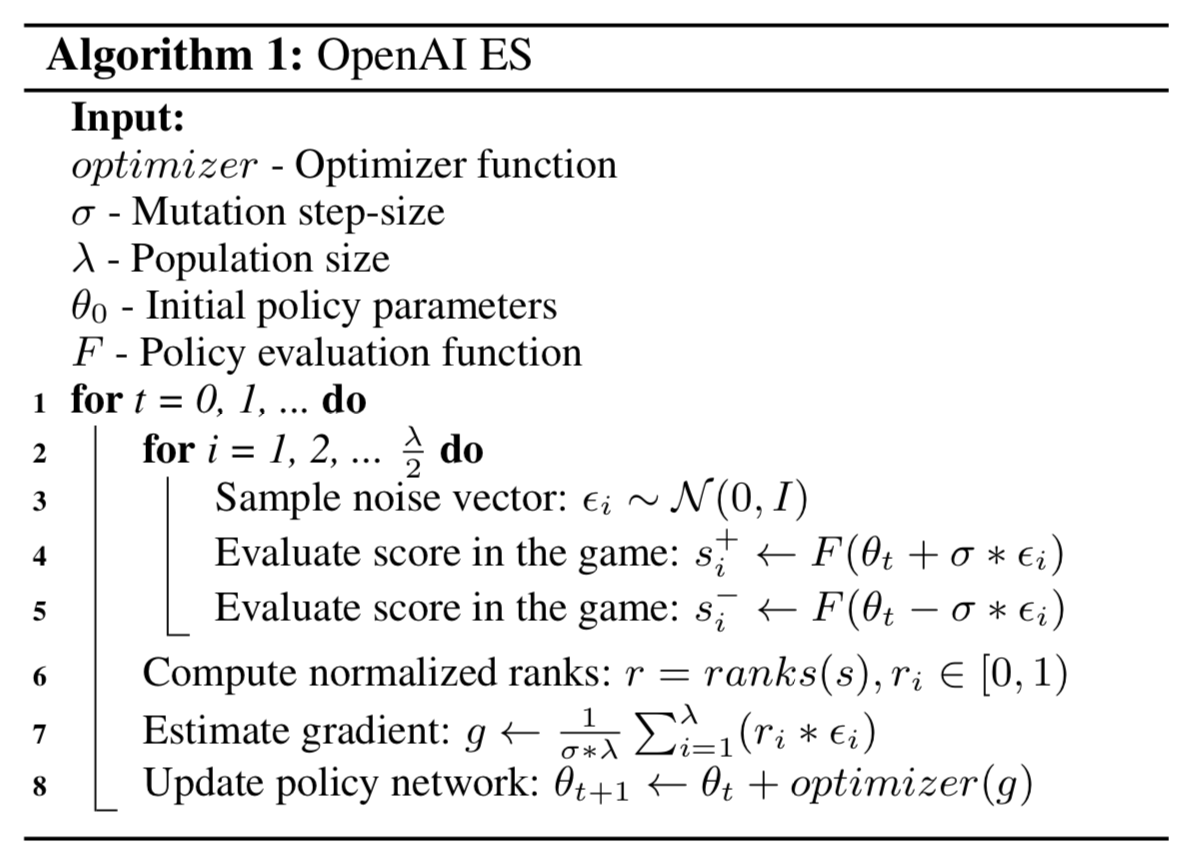
\includegraphics[width=.95\linewidth]{figures/OpenAI_ES.png}
		\caption{OpenAI ES algorithm}
		\label{openai}
\end{subfigure}
\begin{subfigure}{.49\textwidth}
		\centering
		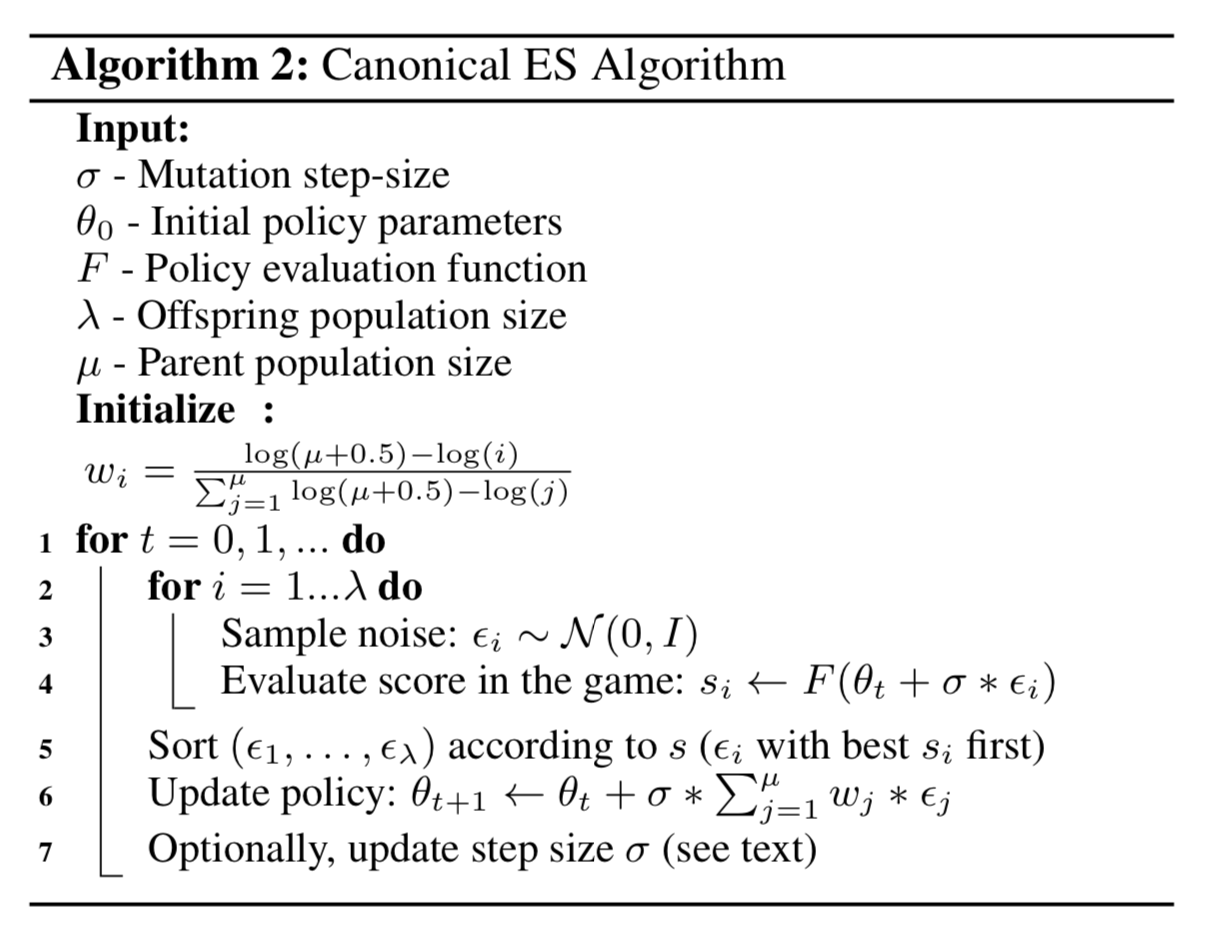
\includegraphics[width=.95\linewidth]{figures/Canonical_ES.png}
		\caption{Canonical ES algorithm}
		\label{canonical}
\end{subfigure}
\caption{Algorithms}
\label{fig:algorithms}
\end{figure}

The Canonical ES [\ref{canonical}] is simpler than OpenAI ES [\ref{openai}] since it does not use mirrored sampling, does not decay the parameters and does not use any advanced optimizer. Also, the step-size adaptation from the description [\ref{canonical}] was removed (fixed step-size was used instead), making it even simpler than typical ES.

The authors compared the performances of these two algorithmsin $8$ different Attari games available in in OpenAI Gym. For the neural network, the architecture used is represented at \cref{fig:nn}. Vitual batch normalization was used by them as well.

About the \textbf{training}: for each game and each ES variant tested, they performed $3$ training runs, each on the roughly equivalent of $800$ CPUs for $5$ hours.

\begin{figure}[ht]
	\begin{center}
		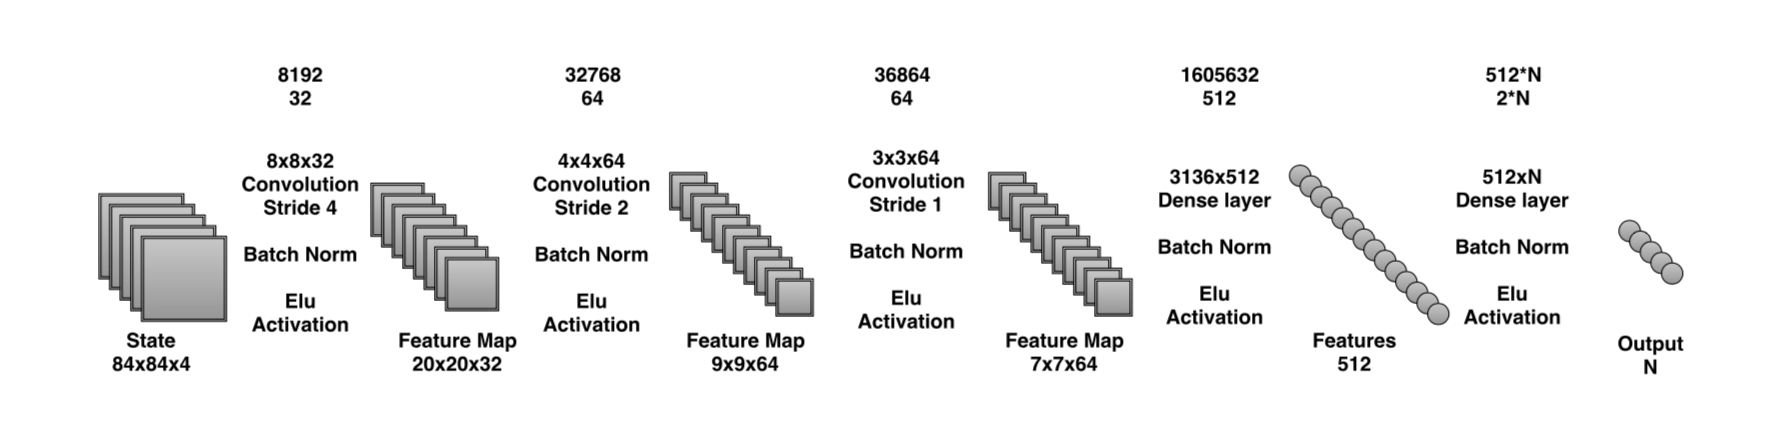
\includegraphics[width=1\columnwidth]{figures/nn.png}
	\end{center}
	\caption{Neural network architecture}
	\label{fig:nn}
\end{figure}

\section{Results}
 \Cref{fig:regions} shows the results found by the authors. The best found values are boldfaced and the values for which the difference is significant across runs  are marked in blue. The algorithm presented by the paper showed improvements between 1 and 5 hours for 16 out of 24 cases but it tends to plateau after extends periods of time. Also, they are not robust to noise in the domain. There is a high variance in the points scored with the same policy for different initial conditions.

\begin{figure}[ht]
	\begin{center}
		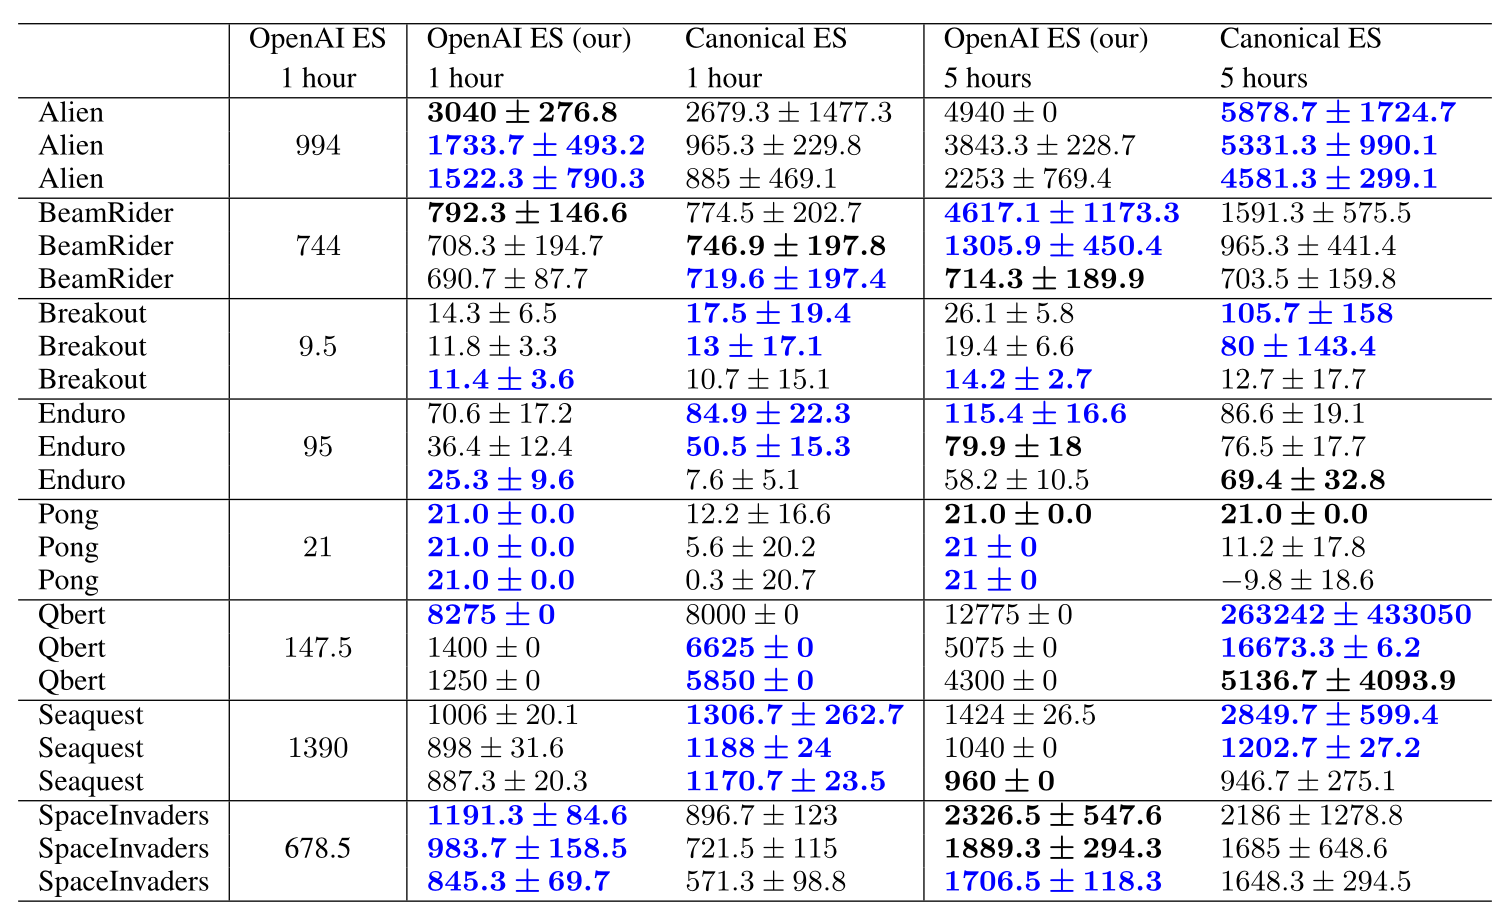
\includegraphics[width=1\columnwidth]{figures/results_table.png}
	\end{center}
	\caption{Results found by the original authors. Available in \cite{DBLP:journals/corr/abs-1802-08842}.}
	\label{fig:regions}
\end{figure}

The visual inspection of the solutions the authors could draft a few conclusions.

For the games Seaquest and Enduro the authors found that the ES converges to suboptimal solutions. In Seaquest, the agent dives and start shooting to left and right, hitting enemies and scoring but it cannot detect the lack of oxygen and dies. In Enduro, the agent steers the car to keep in the middle of the road accelerating but sometimes it bounces back when it hits an opponent. From this visual analysis the author concluded the algorithms got stuck in this suboptimal solutions without a complex behaviour since it gives a much better score than a random approach.

In Qbert, the authors found two interesting solutions. The agent learns to kill itself in order to kill an opponent. More impressively, it learns exploit an in-game bug to gain points, even tough it is not able to consistently exploit this bug. When it fails to exploit the bug it ends up with a low score.

Breakout is a challenging gamer where the ES found a similar solution to RL but its solutions is not very stable. For a few different initial conditions the same agent loses with only a few points.

In both SpaceInvaders and Alien the ES found a strategy that maximizes the score even at the cost of the main game objective. The authors concluded that this is an important difference from the reinforcement learning and this is caused by the fact that, differently from the RL, the ES does not clip the reward during training.

\section{Conclusion}
The authors could conclude based on the work of \cite{salimans2017evolution} that evolution strategies are a viable alternative for deep reinforcement learning. In the top of that, they also concluded  that even a simpler algorithm than the one shown in \cite{salimans2017evolution} can find good solutions. He ends up by proposing future works that combine the strengths of both Evolution Strategies and Reinforcement Learning.
% --------------------------------------------------------------
%                       Bibliography
% --------------------------------------------------------------
\phantomsection
\addcontentsline{toc}{section}{References}
\bibliography{bibliography}
\end{document}
